\section{Answers Lecture 10 \& 11: Bayesian Inference}

\paragraph{\questionref{q:elec-comm-errors}}
Let's work backwards from what we are asked to compute: $\mathbb{P}(\hat S = S)$. Remember that $\hat S$ is actually a function of $v$, and then let's try to find it in terms of probabilities we can find:
\begin{align}
\mathbb P(\hat S(v) = S) &= \mathbb P(\hat S(v) = 1|S=1)\mathbb P(S=1) + \mathbb P(\hat S(v) = 1|S=0)\mathbb P(S=0) \\
&=\mathbb P(\hat S(v) = 1|S=1) \pi + \mathbb P(\hat S(v) = 1|S=0) (1-\pi) \,.
\end{align}
Now we are left to find $\mathbb P(\hat S(v) = s|S=s)$. To find this probability, we will need to understand the function $\hat S(v)$ a bit better.

We know that $\hat S(v) = \argmax_s p(s|v)$, and so it will have a binary output. Let's understand the region where $\hat S(v) = 1$. We start by noting $\hat S(v) = \argmax_s p(s|v) = \argmax_s p(v|s)p(s)$, so we will have $\hat S(v) = 1$ if
\begin{align}
\log p(v|S=1)p(S=1) &> \log p(v|S=0)p(S=0) \\
-\frac{1}{2\sigma^2}(v-1)^2 + \log p &> -\frac{1}{2\sigma^2}v^2 + \log 1-p \\
\frac{1}{2\sigma^2}2v &> \log \frac{1-p}{p} + \frac{1}{2\sigma^2} \\
v &> \sigma^2\log \frac{1-p}{p} + \frac{1}{2} \coloneqq t \,.
\end{align}

This allows us to compute the two probabilities we are after:
\begin{align}
\mathbb P(\hat S(v) = 0|S=0) &= \int_{-\infty}^t \pi(v|S=0)\calcd v &
\mathbb P(\hat S(v) = 1|S=1) &= \int_{t}^\infty \pi(v|S=1)\calcd v \\
&= \int_{-\infty}^t \NormDist{v; 0, \sigma^2} \calcd v & &= \int_t^\infty \NormDist{v; 1, \sigma^2}\calcd v \\
&= \Phi\left(\frac{t}{\sigma}\right) & &= 1-\Phi\left(\frac{t-1}{\sigma}\right)
\end{align}
Here, we did assume that the true noise distribution is equal to the noise distribution we assume in the model, i.e.~$\pi(v|s) = p(v|s)$. This may not be true of all models!

So, overall, we get:
\begin{align}
\mathbb P(\hat S = S) = \pi \left(1-\Phi\left(\frac{t-1}{\sigma}\right)\right) + (1-\pi)\Phi\left(\frac{t}{\sigma}\right)
\end{align}

Although the question is done, let's get a bit more insight by investigating what happens when we vary $p$, for a true frequency $\mathbb P(S = 1) = \pi = 0.6$. In \cref{fig:elec-comm-errors-varyp}, we plot $\mathbb P(\hat S = S)$ for varying $p$. We see that the probability of getting it right is maximised \emph{when our model prior matches the frequency of reality}.

\begin{figure}[h]
\label{fig:elec-comm-errors-varyp}
\centering
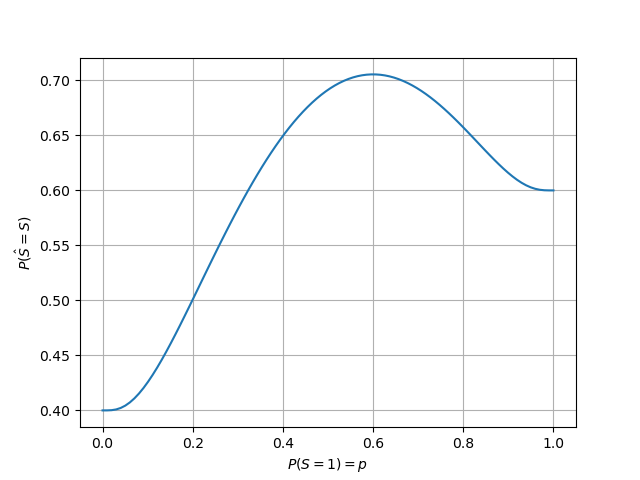
\includegraphics[width=0.8\linewidth]{elec-decoding-errors.png}
\caption{$\mathbb P(\hat S = S)$ for varying $p$.}
\end{figure}
